\subsubsection{Use Cases}
In the following the user types and use cases for the server will be presented. This gives an explanation of which functionality the server should offer, and to whom (that is which user types).
\label{s_actor-goal-list}
In the system we have four kinds of actors:
\begin{description}
	\item [Non-registered user] \hfill \\
		This is the user type with the least options. Only allowed to browse the products, and register to become a customer.
	\item [Customer]  \hfill \\
		The consumer are quite possible the most common user type the service will have. The differences between a customer and a non-registered user is that the customer is able to:
		\begin{itemize}
			\item buy/rent products
			\item download/view products
			\item rate products
		\end{itemize}
	\item [Content provider] \hfill \\
		The content provider are, as the name suggest, the users who is filling the service with products. They can't rent og buy media, but only upload and manage their own products.
	\item [Admin] \hfill \\
		The admin is the most powerful user type, with the power to administrate registered users, content providers and product information.
\end{description}

\subsubsubsection{Use cases}
Maybe this should not be under the server, but only under the client..?\\\\
In the following use cases will be listed for the most relevant use cases. Every use case will have a short description of the scenario the use case is representing, if there are any pre- or postconditions these will be mentioned and then the basic flow for a success scenario will be listed.
\\\\

\textbf{[TODO: Move up usecases from client]}
\textbf{Success scenario: Give dat shit a name} \\
A little tale about it

\begin{tabbing}
\hspace{5mm}\=\hspace{26mm}\=\kill
\>Primary Actor:\> User/user type\\
\>Precondition:\> -.\\
\>Postcondition:\> What is supposed to happen?
\end{tabbing}
\begin{enumerate}
	\item Step 1
	\item Step 2
	\item Step 3
\end{enumerate}
\vspace{3mm}

\subsubsubsection{Use case diagram}
\textbf{[TODO: Should this section be moved up over the use cases?]}
We have produced a use case diagram, see Figure \ref{useCaseImg} p. \pageref{useCaseImg}, which outlines the boundaries of the system, and how the different actors (user types) can interact with the server. 
\begin{figure}[h]
\centering
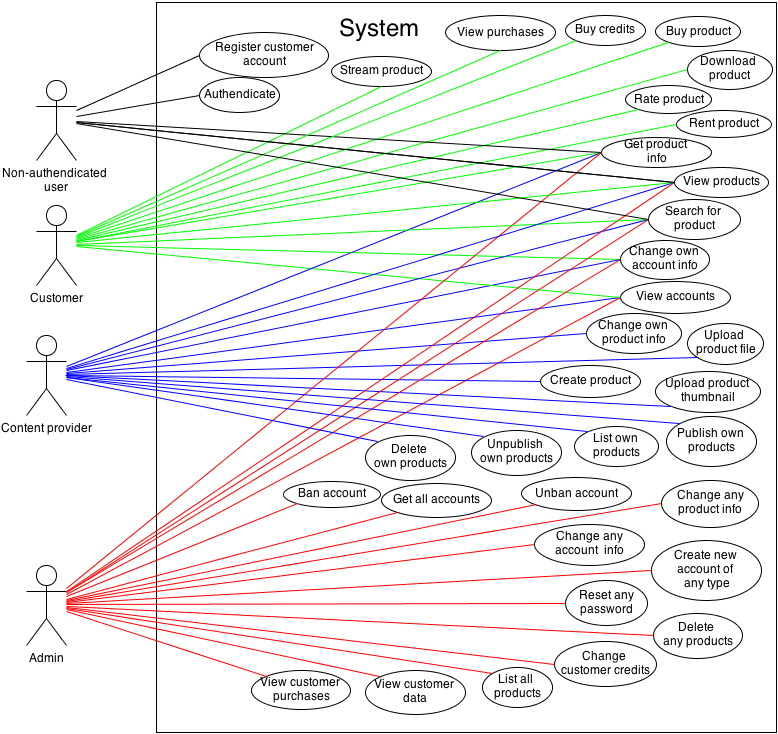
\includegraphics[scale=0.5]{illustrations/UseCaseDiagram.png}
\caption{Use case diagram for our web service}
\label{useCaseImg}
\end{figure}